% Options for packages loaded elsewhere
\PassOptionsToPackage{unicode}{hyperref}
\PassOptionsToPackage{hyphens}{url}
%
\documentclass[
]{article}
\usepackage{amsmath,amssymb}
\usepackage{iftex}
\ifPDFTeX
  \usepackage[T1]{fontenc}
  \usepackage[utf8]{inputenc}
  \usepackage{textcomp} % provide euro and other symbols
\else % if luatex or xetex
  \usepackage{unicode-math} % this also loads fontspec
  \defaultfontfeatures{Scale=MatchLowercase}
  \defaultfontfeatures[\rmfamily]{Ligatures=TeX,Scale=1}
\fi
\usepackage{lmodern}
\ifPDFTeX\else
  % xetex/luatex font selection
\fi
% Use upquote if available, for straight quotes in verbatim environments
\IfFileExists{upquote.sty}{\usepackage{upquote}}{}
\IfFileExists{microtype.sty}{% use microtype if available
  \usepackage[]{microtype}
  \UseMicrotypeSet[protrusion]{basicmath} % disable protrusion for tt fonts
}{}
\makeatletter
\@ifundefined{KOMAClassName}{% if non-KOMA class
  \IfFileExists{parskip.sty}{%
    \usepackage{parskip}
  }{% else
    \setlength{\parindent}{0pt}
    \setlength{\parskip}{6pt plus 2pt minus 1pt}}
}{% if KOMA class
  \KOMAoptions{parskip=half}}
\makeatother
\usepackage{xcolor}
\usepackage[margin=1in]{geometry}
\usepackage{color}
\usepackage{fancyvrb}
\newcommand{\VerbBar}{|}
\newcommand{\VERB}{\Verb[commandchars=\\\{\}]}
\DefineVerbatimEnvironment{Highlighting}{Verbatim}{commandchars=\\\{\}}
% Add ',fontsize=\small' for more characters per line
\usepackage{framed}
\definecolor{shadecolor}{RGB}{248,248,248}
\newenvironment{Shaded}{\begin{snugshade}}{\end{snugshade}}
\newcommand{\AlertTok}[1]{\textcolor[rgb]{0.94,0.16,0.16}{#1}}
\newcommand{\AnnotationTok}[1]{\textcolor[rgb]{0.56,0.35,0.01}{\textbf{\textit{#1}}}}
\newcommand{\AttributeTok}[1]{\textcolor[rgb]{0.13,0.29,0.53}{#1}}
\newcommand{\BaseNTok}[1]{\textcolor[rgb]{0.00,0.00,0.81}{#1}}
\newcommand{\BuiltInTok}[1]{#1}
\newcommand{\CharTok}[1]{\textcolor[rgb]{0.31,0.60,0.02}{#1}}
\newcommand{\CommentTok}[1]{\textcolor[rgb]{0.56,0.35,0.01}{\textit{#1}}}
\newcommand{\CommentVarTok}[1]{\textcolor[rgb]{0.56,0.35,0.01}{\textbf{\textit{#1}}}}
\newcommand{\ConstantTok}[1]{\textcolor[rgb]{0.56,0.35,0.01}{#1}}
\newcommand{\ControlFlowTok}[1]{\textcolor[rgb]{0.13,0.29,0.53}{\textbf{#1}}}
\newcommand{\DataTypeTok}[1]{\textcolor[rgb]{0.13,0.29,0.53}{#1}}
\newcommand{\DecValTok}[1]{\textcolor[rgb]{0.00,0.00,0.81}{#1}}
\newcommand{\DocumentationTok}[1]{\textcolor[rgb]{0.56,0.35,0.01}{\textbf{\textit{#1}}}}
\newcommand{\ErrorTok}[1]{\textcolor[rgb]{0.64,0.00,0.00}{\textbf{#1}}}
\newcommand{\ExtensionTok}[1]{#1}
\newcommand{\FloatTok}[1]{\textcolor[rgb]{0.00,0.00,0.81}{#1}}
\newcommand{\FunctionTok}[1]{\textcolor[rgb]{0.13,0.29,0.53}{\textbf{#1}}}
\newcommand{\ImportTok}[1]{#1}
\newcommand{\InformationTok}[1]{\textcolor[rgb]{0.56,0.35,0.01}{\textbf{\textit{#1}}}}
\newcommand{\KeywordTok}[1]{\textcolor[rgb]{0.13,0.29,0.53}{\textbf{#1}}}
\newcommand{\NormalTok}[1]{#1}
\newcommand{\OperatorTok}[1]{\textcolor[rgb]{0.81,0.36,0.00}{\textbf{#1}}}
\newcommand{\OtherTok}[1]{\textcolor[rgb]{0.56,0.35,0.01}{#1}}
\newcommand{\PreprocessorTok}[1]{\textcolor[rgb]{0.56,0.35,0.01}{\textit{#1}}}
\newcommand{\RegionMarkerTok}[1]{#1}
\newcommand{\SpecialCharTok}[1]{\textcolor[rgb]{0.81,0.36,0.00}{\textbf{#1}}}
\newcommand{\SpecialStringTok}[1]{\textcolor[rgb]{0.31,0.60,0.02}{#1}}
\newcommand{\StringTok}[1]{\textcolor[rgb]{0.31,0.60,0.02}{#1}}
\newcommand{\VariableTok}[1]{\textcolor[rgb]{0.00,0.00,0.00}{#1}}
\newcommand{\VerbatimStringTok}[1]{\textcolor[rgb]{0.31,0.60,0.02}{#1}}
\newcommand{\WarningTok}[1]{\textcolor[rgb]{0.56,0.35,0.01}{\textbf{\textit{#1}}}}
\usepackage{graphicx}
\makeatletter
\def\maxwidth{\ifdim\Gin@nat@width>\linewidth\linewidth\else\Gin@nat@width\fi}
\def\maxheight{\ifdim\Gin@nat@height>\textheight\textheight\else\Gin@nat@height\fi}
\makeatother
% Scale images if necessary, so that they will not overflow the page
% margins by default, and it is still possible to overwrite the defaults
% using explicit options in \includegraphics[width, height, ...]{}
\setkeys{Gin}{width=\maxwidth,height=\maxheight,keepaspectratio}
% Set default figure placement to htbp
\makeatletter
\def\fps@figure{htbp}
\makeatother
\setlength{\emergencystretch}{3em} % prevent overfull lines
\providecommand{\tightlist}{%
  \setlength{\itemsep}{0pt}\setlength{\parskip}{0pt}}
\setcounter{secnumdepth}{-\maxdimen} % remove section numbering
\ifLuaTeX
  \usepackage{selnolig}  % disable illegal ligatures
\fi
\IfFileExists{bookmark.sty}{\usepackage{bookmark}}{\usepackage{hyperref}}
\IfFileExists{xurl.sty}{\usepackage{xurl}}{} % add URL line breaks if available
\urlstyle{same}
\hypersetup{
  pdftitle={Exam 2023},
  hidelinks,
  pdfcreator={LaTeX via pandoc}}

\title{Exam 2023}
\author{}
\date{\vspace{-2.5em}2024-01-23}

\begin{document}
\maketitle

\hypertarget{exercise-1}{%
\section{Exercise 1}\label{exercise-1}}

Let \(X\) be uniform on the unit interval. Let
\(Y | X = x \sim \mathcal{N}(0,x)\).

\hypertarget{section}{%
\subsection{1.}\label{section}}

We can simulate from the joint distribution of \((X,Y)\) by first
simulating from the marginal of \(X\) and then using the conditional
distribution of \(Y\) given \(X\) to simulate from \(Y\). We count the
number of times out of \(n = 10^5\) that \(Y < 1\) to get an estimate of
\(P(Y < 1)\). Recall that \texttt{r} parametrizes the normal
distribution with the standard deviation, so we take the square root of
\(X\) below

\begin{Shaded}
\begin{Highlighting}[]
\FunctionTok{set.seed}\NormalTok{(}\DecValTok{1}\NormalTok{)}
\NormalTok{n }\OtherTok{\textless{}{-}} \FloatTok{10e5}
\NormalTok{X }\OtherTok{\textless{}{-}} \FunctionTok{runif}\NormalTok{(n)}
\NormalTok{Y }\OtherTok{\textless{}{-}} \FunctionTok{rnorm}\NormalTok{(n, }\DecValTok{0}\NormalTok{, }\FunctionTok{sqrt}\NormalTok{(X))}
\FunctionTok{mean}\NormalTok{(Y }\SpecialCharTok{\textless{}} \DecValTok{1}\NormalTok{)}
\end{Highlighting}
\end{Shaded}

\begin{verbatim}
## [1] 0.924313
\end{verbatim}

We see that \(P(Y < 1) \approx 0.924313\).

\hypertarget{section-1}{%
\subsection{2.}\label{section-1}}

By the law of total expectation

\[
E(Y) = E(E(Y|X)) = E(0) = 0
\] And by theorem 3.3

\[
V(Y) = V(E(Y|X)) + E(V(Y|X)) = V(0) + E(X) = 1/2
\]

\hypertarget{section-2}{%
\subsection{3.}\label{section-2}}

Since \(X\) and \(Y | X = x\) both have densities w.r.t. the Lebesgue
measure which is \(\sigma\)-finite, it follows from theorem 2.1 that
\((X,Y)\) has joint density \(h\) w.r.t. the 2-dimensional lebesgue
measure. We have that \[
h(x,y) = q(x) \cdot g_x(y) = 1_{[0,1]}(x) \cdot \frac{1}{\sqrt{2\pi x}} \exp(-\frac{y^2}{2x} )
\] It now follows from theorem 2.2 that the conditional distribution of
\(X | y = t\) exists and has density w.r.t. the Lebesgue measure which
satisfies by \[
q_y(x) \propto h(x,y) = 1_{[0,1]}(x) \cdot \frac{1}{\sqrt{2\pi x}} \exp(-\frac{y^2}{2x} ) \propto 1_{(0,1)}(x) \cdot x^{-1/2} \exp(-\frac{y^2}{2x} )
\]

\hypertarget{section-3}{%
\subsection{4.}\label{section-3}}

Consider the case \(Y = 0\). Then \[
q_0(x) \propto 1_{(0,1)}(x) \cdot x^{-1/2} \exp(0) = 1_{(0,1)}(x) \cdot x^{-1/2}
\] Recall that the \(\chi^2(1)\) has density \[
f(x) = \frac{1}{2^{1/2}\Gamma(1/2)} x^{-1/2} \exp(-x/2) 1_{(0,\infty)}(x) = C x^{-1/2} \exp(-x/2) 1_{(0,\infty)}(x)
\] Letting \(C = \frac{1}{2^{1/2}\Gamma(1/2)}\). We can clearly sample
from the \(\chi^2(1)\) distribution, and noting that for some constant
\(M > 0\) \[
1_{(0,1)}(x) \cdot x^{-1/2} \leq M \cdot C \cdot x^{-1/2} \exp(-x/2) 1_{(0,\infty)}(x) \Leftrightarrow 1_{(0,1)}(x) \leq M \cdot C \cdot  \exp(-x/2) 1_{(0,\infty)}(x)
\] If \(x \geq 1\) the inequality trivially holds. If \(0 \leq x < 1\)
we have that \(\exp(-1/2) < \exp(-x/2) \leq 1\), hence if we want the
inequality to hold for all \(x \in (0,1)\) we have to solve \[
1 \leq M \cdot C \cdot \exp(-1/2) \Leftrightarrow \frac{\exp(1/2)}{C} \leq M 
\] The value \(M\) that maximizes the acceptance probability is the
\(M\) that ensures equality in the above \[
M = \frac{\exp(1/2)}{C} = 2^{1/2}\Gamma(1/2) \exp(1/2)
\] With this choice of \(M\) we obtain that \[
1_{(0,1)}(x) \cdot x^{-1/2} \leq M \cdot f(x)
\] Which shows that we can use rejecetion sampling with \(\chi^2(1)\) as
the proposal to sample from \(Q_0\). The probability that a sample
\(x^*\) will be accepted is \[
\alpha = \frac{1_{(0,1)}(x^*) \cdot (x^*)^{-1/2}}{Mf(x^*)}
\] Which could probably be simplifed. We simulate from \(Q_0\) and
compute \(E(Y| X= 0 )\).

\begin{Shaded}
\begin{Highlighting}[]
\FunctionTok{set.seed}\NormalTok{(}\DecValTok{1}\NormalTok{)}
\NormalTok{C }\OtherTok{\textless{}{-}} \DecValTok{1}\SpecialCharTok{/}\NormalTok{(}\DecValTok{2}\SpecialCharTok{\^{}}\NormalTok{(}\DecValTok{1}\SpecialCharTok{/}\DecValTok{2}\NormalTok{)}\SpecialCharTok{*}\FunctionTok{gamma}\NormalTok{(}\DecValTok{1}\SpecialCharTok{/}\DecValTok{2}\NormalTok{))}
\NormalTok{M }\OtherTok{\textless{}{-}} \FunctionTok{exp}\NormalTok{(}\DecValTok{1}\SpecialCharTok{/}\DecValTok{2}\NormalTok{)}\SpecialCharTok{/}\NormalTok{C}
\NormalTok{proposal }\OtherTok{\textless{}{-}} \ControlFlowTok{function}\NormalTok{(x)\{}
  \FunctionTok{dchisq}\NormalTok{(x, }\DecValTok{1}\NormalTok{)}
\NormalTok{\}}
\NormalTok{target }\OtherTok{\textless{}{-}} \ControlFlowTok{function}\NormalTok{(x)\{}
\NormalTok{  (x}\SpecialCharTok{\textgreater{}}\DecValTok{0}\NormalTok{)}\SpecialCharTok{*}\NormalTok{(x}\SpecialCharTok{\textless{}}\DecValTok{1}\NormalTok{)}\SpecialCharTok{*}\NormalTok{x}\SpecialCharTok{\^{}}\NormalTok{(}\SpecialCharTok{{-}}\DecValTok{1}\SpecialCharTok{/}\DecValTok{2}\NormalTok{)}
\NormalTok{\}}
\NormalTok{sample\_dist }\OtherTok{\textless{}{-}} \ControlFlowTok{function}\NormalTok{(n)\{}
  \FunctionTok{rchisq}\NormalTok{(}\AttributeTok{n=}\NormalTok{n, }\AttributeTok{df =} \DecValTok{1}\NormalTok{)}
\NormalTok{\}}

\NormalTok{rejection\_sample }\OtherTok{\textless{}{-}} \ControlFlowTok{function}\NormalTok{(M, proposal, target, sample\_dist, }\AttributeTok{print\_acceptance =} \ConstantTok{TRUE}\NormalTok{)\{}
\NormalTok{  theta\_star }\OtherTok{\textless{}{-}} \FunctionTok{sample\_dist}\NormalTok{(}\AttributeTok{n =} \FloatTok{1e6}\NormalTok{)}
\NormalTok{  U }\OtherTok{\textless{}{-}} \FunctionTok{runif}\NormalTok{(}\FloatTok{1e6}\NormalTok{)}
\NormalTok{  alpha }\OtherTok{\textless{}{-}} \FunctionTok{target}\NormalTok{(theta\_star)}\SpecialCharTok{/}\NormalTok{(M}\SpecialCharTok{*}\FunctionTok{proposal}\NormalTok{(theta\_star))}
\NormalTok{  idx }\OtherTok{\textless{}{-}}\NormalTok{ (U }\SpecialCharTok{\textless{}=}\NormalTok{ alpha)}
  \ControlFlowTok{if}\NormalTok{(print\_acceptance)\{}
    \FunctionTok{cat}\NormalTok{(}\StringTok{"Acceptance rate is: "}\NormalTok{, }\FunctionTok{sum}\NormalTok{(idx)}\SpecialCharTok{/}\FloatTok{1e6}\NormalTok{)}
\NormalTok{  \}}
  \FunctionTok{return}\NormalTok{(theta\_star[idx])}
\NormalTok{\}}
\NormalTok{X }\OtherTok{\textless{}{-}} \FunctionTok{rejection\_sample}\NormalTok{(M, }\AttributeTok{proposal =}\NormalTok{ proposal, }\AttributeTok{target =}\NormalTok{ target, }\AttributeTok{sample\_dist =}\NormalTok{ sample\_dist)}
\end{Highlighting}
\end{Shaded}

\begin{verbatim}
## Acceptance rate is:  0.484515
\end{verbatim}

\begin{Shaded}
\begin{Highlighting}[]
\FunctionTok{mean}\NormalTok{(X)}
\end{Highlighting}
\end{Shaded}

\begin{verbatim}
## [1] 0.3334866
\end{verbatim}

We get \(E(Y|X = 0) \approx 0.3329909\).

\textbf{COMMENT}: It is actually not necessary to carry around the
constant \(C\) for the \(\chi^2\) distribution in the above. If only
calculating up to proportionality it will cancel when computing
\(\alpha\). This would mean that the sample\_dist parameter above should
be the unnormalized proposal instead. Accordingly \(M\) would change
from \(M = \exp(1/2)/C\) to \(M = \exp(1/2)\).

\hypertarget{exercise-2}{%
\section{Exercise 2}\label{exercise-2}}

We load the data and add \(\log(SOC)\) as a variable in the dataset.

\begin{Shaded}
\begin{Highlighting}[]
\FunctionTok{rm}\NormalTok{(}\AttributeTok{list =} \FunctionTok{ls}\NormalTok{())}
\FunctionTok{load}\NormalTok{(}\StringTok{"april22.Rdata"}\NormalTok{)}
\NormalTok{SOCdata }\OtherTok{\textless{}{-}}\NormalTok{ SOCdata }\SpecialCharTok{\%\textgreater{}\%} \FunctionTok{tibble}\NormalTok{() }\SpecialCharTok{\%\textgreater{}\%} \FunctionTok{mutate}\NormalTok{(}\AttributeTok{log\_SOC =} \FunctionTok{log}\NormalTok{(SOC))}
\end{Highlighting}
\end{Shaded}

\hypertarget{section-4}{%
\subsection{1.}\label{section-4}}

It is most appropriate to use plant as a random factor, as we want to
view the plants as a random sample from the population of plants, such
that we can draw inference for the population of plants as a whole and
not just about the specific plants in the dataset. Furthermore,
measurements from the same plant is likely correlated, so it would be
inappropriate to model observations from the same plant as independent.

In this experiment it is most appropriate to model block as a fixed
effect rather than a random effect because the `were deliberately chosen
such that they represent three different soil conditions'. This means
that we are not interested in viewing blocks as a sample from the
`population of blocks', but rather we may be interested in saying
something about the soil conditions effect on soil organic carbon.
Hence, we should model it as a fixed effect.

We fit \texttt{M1} and \texttt{M2}. And make residual plots. Note that
the plot on the left is the one were SOC is not log-transformed and the
one on the right is the log-transformed version

\begin{Shaded}
\begin{Highlighting}[]
\NormalTok{M1 }\OtherTok{\textless{}{-}} \FunctionTok{lmer}\NormalTok{(SOC }\SpecialCharTok{\textasciitilde{}}\NormalTok{ Treat }\SpecialCharTok{{-}}\DecValTok{1} \SpecialCharTok{+}\NormalTok{ Block}\SpecialCharTok{*}\NormalTok{DepthFac }\SpecialCharTok{+}\NormalTok{ (}\DecValTok{1}\SpecialCharTok{|}\NormalTok{Plant), }\AttributeTok{data=}\NormalTok{SOCdata)}
\end{Highlighting}
\end{Shaded}

\begin{verbatim}
## boundary (singular) fit: see help('isSingular')
\end{verbatim}

\begin{Shaded}
\begin{Highlighting}[]
\NormalTok{M2 }\OtherTok{\textless{}{-}} \FunctionTok{lmer}\NormalTok{(log\_SOC }\SpecialCharTok{\textasciitilde{}}\NormalTok{ Treat }\SpecialCharTok{{-}}\DecValTok{1} \SpecialCharTok{+}\NormalTok{ Block}\SpecialCharTok{*}\NormalTok{DepthFac }\SpecialCharTok{+}\NormalTok{ (}\DecValTok{1}\SpecialCharTok{|}\NormalTok{Plant), }\AttributeTok{data=}\NormalTok{SOCdata)}
\NormalTok{gridExtra}\SpecialCharTok{::}\FunctionTok{grid.arrange}\NormalTok{(}
  \FunctionTok{plot}\NormalTok{(M1),}
  \FunctionTok{plot}\NormalTok{(M2),}
  \AttributeTok{ncol =} \DecValTok{2}
\NormalTok{)}
\end{Highlighting}
\end{Shaded}

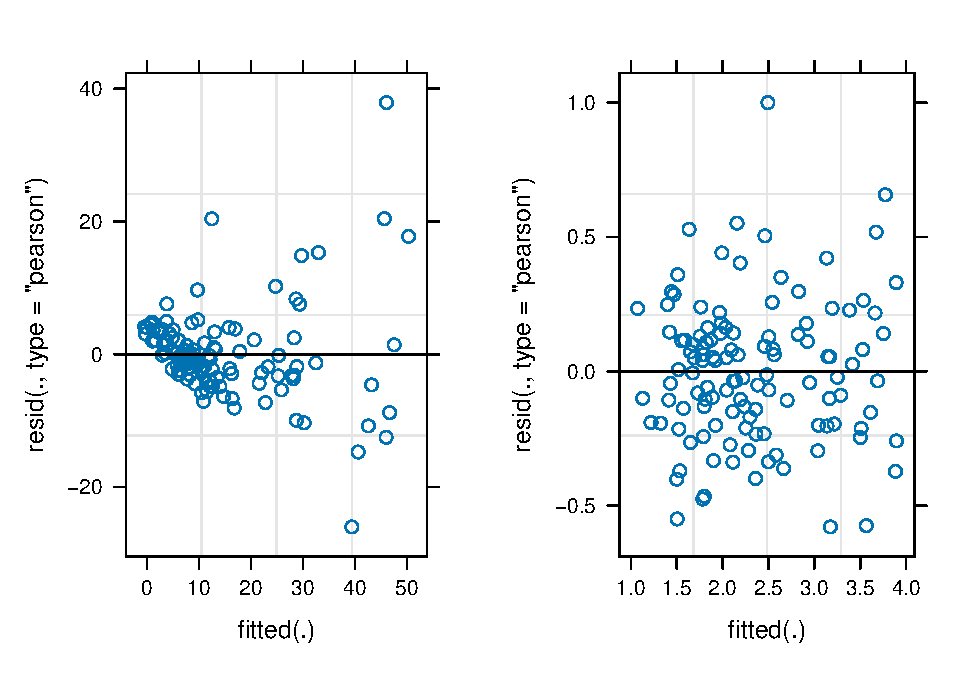
\includegraphics{besvarels_files/figure-latex/unnamed-chunk-4-1.pdf}

We see a clear pattern in the residual plot from the non-logtransformed
model. There is clear overdispersion/variance inhomogeneity as variance
seems to increase with fitted values. The mean value structure also
looks a bit off for small fitted values as there seems to be a downward
trend in the residuals for small fitted values. The residual after
log-transformation is much nicer. There is no sign of variance
inhomogeneity and the mean structure also seems good.

\hypertarget{section-5}{%
\subsection{2.}\label{section-5}}

We print a summary of \texttt{M2}

\begin{Shaded}
\begin{Highlighting}[]
\FunctionTok{summary}\NormalTok{(M2)}
\end{Highlighting}
\end{Shaded}

\begin{verbatim}
## Linear mixed model fit by REML ['lmerMod']
## Formula: log_SOC ~ Treat - 1 + Block * DepthFac + (1 | Plant)
##    Data: SOCdata
## 
## REML criterion at convergence: 106.7
## 
## Scaled residuals: 
##     Min      1Q  Median      3Q     Max 
## -1.8936 -0.6336 -0.0315  0.4621  3.2692 
## 
## Random effects:
##  Groups   Name        Variance Std.Dev.
##  Plant    (Intercept) 0.02366  0.1538  
##  Residual             0.09356  0.3059  
## Number of obs: 120, groups:  Plant, 30
## 
## Fixed effects:
##                    Estimate Std. Error t value
## TreatA              3.19221    0.16074  19.859
## TreatB              3.50934    0.16074  21.832
## TreatC              3.49745    0.16074  21.758
## TreatD              3.21403    0.16074  19.995
## TreatE              3.37264    0.16074  20.982
## TreatF              3.47085    0.16074  21.593
## TreatG              3.07392    0.16074  19.124
## TreatH              3.23905    0.16074  20.151
## TreatI              3.08815    0.16074  19.212
## TreatControl        2.86858    0.16074  17.846
## Blockb              0.00574    0.15312   0.037
## Blockc              0.43173    0.15312   2.820
## DepthFac25         -0.58466    0.13679  -4.274
## DepthFac55         -1.05250    0.13679  -7.694
## DepthFac100        -1.61424    0.13679 -11.801
## Blockb:DepthFac25  -0.43965    0.19345  -2.273
## Blockc:DepthFac25  -0.80589    0.19345  -4.166
## Blockb:DepthFac55  -0.35552    0.19345  -1.838
## Blockc:DepthFac55  -0.79753    0.19345  -4.123
## Blockb:DepthFac100 -0.07874    0.19345  -0.407
## Blockc:DepthFac100 -0.48591    0.19345  -2.512
\end{verbatim}

\begin{verbatim}
## 
## Correlation matrix not shown by default, as p = 21 > 12.
## Use print(x, correlation=TRUE)  or
##     vcov(x)        if you need it
\end{verbatim}

We see that the residual variance is estimated to
\(\hat{\sigma} = 0.09356\) and the within plant variance is estimated to
\(\hat{\sigma}_p = 0.02366\). This implies that \[
\hat{V}(Y_1) = \hat{\sigma}^2 + \hat{\sigma}^2_p = 0.02366+ 0.09356 = 0.11722
\] If we have another measurement from the same plant but at different
depths, an estimate for \(\rho(Y_1, Y_2)\) is \[
\hat{\rho}(Y_1, Y_2) = \frac{\hat{\sigma}^2_p}{\hat{\sigma}^2 + \hat{\sigma}^2_p} = \frac{0.02366}{0.11722} = 0.2018427
\]

\hypertarget{section-6}{%
\subsection{3}\label{section-6}}

Consider the models \texttt{M2} and \texttt{M3}. When we test the model
reduction from \texttt{M2} to \texttt{M3} we are testing the hypothesis
\[
H_0: EY \in  L_{Block \, \times DepthFac}
\] Against the larger model \[
EY \in L_{Treat} + L_{Block \, \times DepthFac}
\]

We do this by computing a Likelihood ratio test statistics. Notice that
we have 10 treatments, so we should compare the likelihood ratio test
statistic to a \(\chi^2 (10-1)\) distribution, i.e.~a \(\chi^2\)
distribution with \(9\) degrees of freedom. We carry out the test with
the \texttt{PBModComp} function from \texttt{pbkrtest}

\begin{Shaded}
\begin{Highlighting}[]
\NormalTok{M3 }\OtherTok{\textless{}{-}} \FunctionTok{lmer}\NormalTok{(log\_SOC }\SpecialCharTok{\textasciitilde{}}\NormalTok{ Block}\SpecialCharTok{*}\NormalTok{DepthFac }\SpecialCharTok{+}\NormalTok{ (}\DecValTok{1}\SpecialCharTok{|}\NormalTok{Plant), }\AttributeTok{data=}\NormalTok{SOCdata)}
\FunctionTok{PBmodcomp}\NormalTok{(M2, M3, }\AttributeTok{nsim =} \DecValTok{1000}\NormalTok{)}
\end{Highlighting}
\end{Shaded}

\begin{verbatim}
## Warning in checkConv(attr(opt, "derivs"), opt$par, ctrl = control$checkConv, :
## Model failed to converge with max|grad| = 0.00265799 (tol = 0.002, component 1)
\end{verbatim}

\begin{verbatim}
## Warning in checkConv(attr(opt, "derivs"), opt$par, ctrl = control$checkConv, :
## Model failed to converge with max|grad| = 0.00238568 (tol = 0.002, component 1)
\end{verbatim}

\begin{verbatim}
## Bootstrap test; time: 25.22 sec; samples: 1000; extremes: 28;
## large : log_SOC ~ Treat - 1 + Block * DepthFac + (1 | Plant)
## log_SOC ~ Block * DepthFac + (1 | Plant)
##         stat df  p.value   
## LRT    26.46  9 0.001717 **
## PBtest 26.46    0.028971 * 
## ---
## Signif. codes:  0 '***' 0.001 '**' 0.01 '*' 0.05 '.' 0.1 ' ' 1
\end{verbatim}

We see that we get a LRT statistic of 26.46, and the corresponding
\(p\)-value is 0.001717. This is significant, and hence we reject
\(H_0\) - and even fairly strongly so.

\hypertarget{section-7}{%
\subsection{4.}\label{section-7}}

In question 3, we actually also simulated 1000 LRT statistics from the
model. From these we get a \(p\)-value of 0.028971 This is still
significant at a \(5\%\) level, but it is an order of magnitude larger
than the \(\chi^2\)-approximation and all in all much less convicing,
even though we would still reject \(H_0\).

\hypertarget{section-8}{%
\subsection{5.}\label{section-8}}

Consider \texttt{M2}. Let
\(\alpha_A, \cdots \alpha_I, \alpha_{control}\) be the first ten
parameters of the model and let
\(\delta = \frac{1}{9} (alpha_A + \cdots + \alpha_I) - \alpha_{control}\).
That is, \(\delta\) is the average of the log-SOC for giving some
treatment subtracted with the log-SOC level for the control group.
Hence, \(\delta\) can be interpreted as the average effect (change
relative to control) of giving some treatment. We compute an estimate
for \(\delta\).

\begin{Shaded}
\begin{Highlighting}[]
\NormalTok{(}\FunctionTok{mean}\NormalTok{(}\FunctionTok{fixef}\NormalTok{(M2)[}\DecValTok{1}\SpecialCharTok{:}\DecValTok{9}\NormalTok{]) }\SpecialCharTok{{-}} \FunctionTok{fixef}\NormalTok{(M2)[}\DecValTok{10}\NormalTok{]) }\SpecialCharTok{\%\textgreater{}\%} \FunctionTok{unname}\NormalTok{()}
\end{Highlighting}
\end{Shaded}

\begin{verbatim}
## [1] 0.4267139
\end{verbatim}

And so \(\hat{\delta} = 0.4267139\). Notice that we could also have
computed this as \[
A^T \begin{pmatrix} \alpha_A & \alpha_B & \cdots &  \alpha_I  & \alpha_{control} \end{pmatrix}
\]

\[
A= \begin{pmatrix} 1/9 \\ 1/9  \\  \vdots \\  -1 \end{pmatrix}
\] Let \(\hat{\Sigma}\) be the estimated covariance matrix for the
\(\alpha\) estimates. Per the above, and since the estimates has a
normal distribution under the model assumptions, we can compute an
estimate of the variance for \(\delta\) as \[
\hat{V}(\hat{\delta}) = A^T \hat{\Sigma} A
\] And so an estimate for the standard error is

\begin{Shaded}
\begin{Highlighting}[]
\NormalTok{A }\OtherTok{\textless{}{-}} \FunctionTok{matrix}\NormalTok{(}\FunctionTok{c}\NormalTok{(}\FunctionTok{rep}\NormalTok{(}\DecValTok{1}\SpecialCharTok{/}\DecValTok{9}\NormalTok{,}\DecValTok{9}\NormalTok{),}\SpecialCharTok{{-}}\DecValTok{1}\NormalTok{),}\DecValTok{1}\NormalTok{,}\DecValTok{10}\NormalTok{)}
\FunctionTok{sqrt}\NormalTok{(A }\SpecialCharTok{\%*\%} \FunctionTok{vcov}\NormalTok{(M2)[}\DecValTok{1}\SpecialCharTok{:}\DecValTok{10}\NormalTok{,}\DecValTok{1}\SpecialCharTok{:}\DecValTok{10}\NormalTok{] }\SpecialCharTok{\%*\%} \FunctionTok{t}\NormalTok{(A))[}\DecValTok{1}\NormalTok{,}\DecValTok{1}\NormalTok{]}
\end{Highlighting}
\end{Shaded}

\begin{verbatim}
## [1] 0.1320083
\end{verbatim}

And so \[
\hat{SE}(\hat{\delta}) = 0.1320083
\]

\hypertarget{section-9}{%
\subsection{6.}\label{section-9}}

Consider \texttt{M4}

\begin{Shaded}
\begin{Highlighting}[]
\NormalTok{M4 }\OtherTok{\textless{}{-}} \FunctionTok{lmer}\NormalTok{(log\_SOC }\SpecialCharTok{\textasciitilde{}}\NormalTok{ Treat2 }\SpecialCharTok{+}\NormalTok{ Block}\SpecialCharTok{*}\NormalTok{DepthFac }\SpecialCharTok{+}\NormalTok{ (}\DecValTok{1}\SpecialCharTok{|}\NormalTok{Treat) }\SpecialCharTok{+}\NormalTok{ (}\DecValTok{1}\SpecialCharTok{|}\NormalTok{Plant),}
\AttributeTok{data=}\NormalTok{SOCdata)}
\end{Highlighting}
\end{Shaded}

In this model, the estimate for \texttt{Treat2} is exactly the expected
difference in log(SOC) between an average EFB treatment and control.
Looking at the summary we see that

\begin{Shaded}
\begin{Highlighting}[]
\FunctionTok{summary}\NormalTok{(M4)}
\end{Highlighting}
\end{Shaded}

\begin{verbatim}
## Linear mixed model fit by REML ['lmerMod']
## Formula: log_SOC ~ Treat2 + Block * DepthFac + (1 | Treat) + (1 | Plant)
##    Data: SOCdata
## 
## REML criterion at convergence: 103.4
## 
## Scaled residuals: 
##     Min      1Q  Median      3Q     Max 
## -1.9879 -0.6150  0.0304  0.5284  3.3361 
## 
## Random effects:
##  Groups   Name        Variance Std.Dev.
##  Plant    (Intercept) 0.02366  0.1538  
##  Treat    (Intercept) 0.01379  0.1174  
##  Residual             0.09356  0.3059  
## Number of obs: 120, groups:  Plant, 30; Treat, 10
## 
## Fixed effects:
##                    Estimate Std. Error t value
## (Intercept)         2.86858    0.19907  14.410
## Treat2EFB           0.42671    0.18097   2.358
## Blockb              0.00574    0.15312   0.037
## Blockc              0.43173    0.15312   2.820
## DepthFac25         -0.58466    0.13679  -4.274
## DepthFac55         -1.05250    0.13679  -7.694
## DepthFac100        -1.61424    0.13679 -11.801
## Blockb:DepthFac25  -0.43965    0.19345  -2.273
## Blockc:DepthFac25  -0.80589    0.19345  -4.166
## Blockb:DepthFac55  -0.35552    0.19345  -1.838
## Blockc:DepthFac55  -0.79753    0.19345  -4.123
## Blockb:DepthFac100 -0.07874    0.19345  -0.407
## Blockc:DepthFac100 -0.48591    0.19345  -2.512
\end{verbatim}

\begin{verbatim}
## 
## Correlation matrix not shown by default, as p = 13 > 12.
## Use print(x, correlation=TRUE)  or
##     vcov(x)        if you need it
\end{verbatim}

Hence our estimate \(\hat{\delta}'\) for the expected difference in
log(SOC) between an average EFB treatment and control is thus \[
\hat{\delta}' = 0.42671 
\] and the associated standard error is \[
\hat{SE}(\hat{\delta}') = 0.18097 
\]

Notice that the estimate is exactly the same due to the balanced design,
but that the standard error is know higher, likely due to the fact that
we have included treatment as a random effect. If we fit the model with
\texttt{lmerTest} we get a \(p\)-value from \(t\)-distribution for the
\(\hat{\delta}'\) estimate

\begin{Shaded}
\begin{Highlighting}[]
\NormalTok{lmerTest}\SpecialCharTok{::}\FunctionTok{lmer}\NormalTok{(log\_SOC }\SpecialCharTok{\textasciitilde{}}\NormalTok{ Treat2 }\SpecialCharTok{+}\NormalTok{ Block}\SpecialCharTok{*}\NormalTok{DepthFac }\SpecialCharTok{+}\NormalTok{ (}\DecValTok{1}\SpecialCharTok{|}\NormalTok{Treat) }\SpecialCharTok{+}\NormalTok{ (}\DecValTok{1}\SpecialCharTok{|}\NormalTok{Plant),}
\AttributeTok{data=}\NormalTok{SOCdata) }\SpecialCharTok{\%\textgreater{}\%} \FunctionTok{summary}\NormalTok{()}
\end{Highlighting}
\end{Shaded}

\begin{verbatim}
## Linear mixed model fit by REML. t-tests use Satterthwaite's method [
## lmerModLmerTest]
## Formula: log_SOC ~ Treat2 + Block * DepthFac + (1 | Treat) + (1 | Plant)
##    Data: SOCdata
## 
## REML criterion at convergence: 103.4
## 
## Scaled residuals: 
##     Min      1Q  Median      3Q     Max 
## -1.9879 -0.6150  0.0304  0.5284  3.3361 
## 
## Random effects:
##  Groups   Name        Variance Std.Dev.
##  Plant    (Intercept) 0.02366  0.1538  
##  Treat    (Intercept) 0.01379  0.1174  
##  Residual             0.09356  0.3059  
## Number of obs: 120, groups:  Plant, 30; Treat, 10
## 
## Fixed effects:
##                    Estimate Std. Error       df t value Pr(>|t|)    
## (Intercept)         2.86858    0.19907 14.30854  14.410 6.47e-10 ***
## Treat2EFB           0.42671    0.18097  7.99980   2.358  0.04611 *  
## Blockb              0.00574    0.15312 74.77081   0.037  0.97020    
## Blockc              0.43173    0.15312 74.77081   2.820  0.00615 ** 
## DepthFac25         -0.58466    0.13679 81.00000  -4.274 5.20e-05 ***
## DepthFac55         -1.05250    0.13679 81.00000  -7.694 3.00e-11 ***
## DepthFac100        -1.61424    0.13679 81.00000 -11.801  < 2e-16 ***
## Blockb:DepthFac25  -0.43965    0.19345 81.00000  -2.273  0.02570 *  
## Blockc:DepthFac25  -0.80589    0.19345 81.00000  -4.166 7.71e-05 ***
## Blockb:DepthFac55  -0.35552    0.19345 81.00000  -1.838  0.06977 .  
## Blockc:DepthFac55  -0.79753    0.19345 81.00000  -4.123 9.00e-05 ***
## Blockb:DepthFac100 -0.07874    0.19345 81.00000  -0.407  0.68506    
## Blockc:DepthFac100 -0.48591    0.19345 81.00000  -2.512  0.01400 *  
## ---
## Signif. codes:  0 '***' 0.001 '**' 0.01 '*' 0.05 '.' 0.1 ' ' 1
\end{verbatim}

\begin{verbatim}
## 
## Correlation matrix not shown by default, as p = 13 > 12.
## Use print(x, correlation=TRUE)  or
##     vcov(x)        if you need it
\end{verbatim}

And we see that the effect of EFB treatment is borderline significant at
the \(5\%\) level. We can also do a likelihood ratio test (with both
simulated and the \(\chi^2(1)\) approximation) using \texttt{PBmodComp}
of the same hypothesis:

\begin{Shaded}
\begin{Highlighting}[]
\NormalTok{M4\_small }\OtherTok{\textless{}{-}} \FunctionTok{lmer}\NormalTok{(log\_SOC }\SpecialCharTok{\textasciitilde{}}\NormalTok{ Block}\SpecialCharTok{*}\NormalTok{DepthFac }\SpecialCharTok{+}\NormalTok{ (}\DecValTok{1}\SpecialCharTok{|}\NormalTok{Treat) }\SpecialCharTok{+}\NormalTok{ (}\DecValTok{1}\SpecialCharTok{|}\NormalTok{Plant),}
\AttributeTok{data=}\NormalTok{SOCdata)}

\FunctionTok{PBmodcomp}\NormalTok{(M4, M4\_small)}
\end{Highlighting}
\end{Shaded}

\begin{verbatim}
## Warning in checkConv(attr(opt, "derivs"), opt$par, ctrl = control$checkConv, :
## Model failed to converge with max|grad| = 0.00207362 (tol = 0.002, component 1)
\end{verbatim}

\begin{verbatim}
## Bootstrap test; time: 30.30 sec; samples: 1000; extremes: 36;
## large : log_SOC ~ Treat2 + Block * DepthFac + (1 | Treat) + (1 | Plant)
## log_SOC ~ Block * DepthFac + (1 | Treat) + (1 | Plant)
##          stat df p.value  
## LRT    5.2767  1 0.02161 *
## PBtest 5.2767    0.03696 *
## ---
## Signif. codes:  0 '***' 0.001 '**' 0.01 '*' 0.05 '.' 0.1 ' ' 1
\end{verbatim}

We see that the \(p\)-value corresponding to the \(\chi^2(1)\) is around
the same level as with the \(t\)-test. The \(p\)-value from the
simulated LRT statistics seems to agrees. All in all there is some
evidence that the EFB treatment works, but it is not crystal clear.

\hypertarget{section-10}{%
\subsection{7.}\label{section-10}}

We estimate \(\rho\) the same as we did in question 2, namely \[
\hat{\rho}(Y_1, Y_2) = \frac{\hat{\sigma}^2_p}{\hat{\sigma}^2 + \hat{\sigma}^2_p} 
\] We do this for all the simulated values from the posterior
distribution, and compute a 95\% credible interval by taking quantiles
in this distribution. We compute posterior mean by taking the mean for
the simulated values of \(\rho\):

\begin{Shaded}
\begin{Highlighting}[]
\NormalTok{brmSim2 }\SpecialCharTok{\%\textgreater{}\%} \FunctionTok{tibble}\NormalTok{() }\SpecialCharTok{\%\textgreater{}\%} 
  \FunctionTok{select}\NormalTok{(sd\_Plant\_\_Intercept,sigma) }\SpecialCharTok{\%\textgreater{}\%} 
  \FunctionTok{mutate}\NormalTok{(}\AttributeTok{rho =}\NormalTok{ sd\_Plant\_\_Intercept}\SpecialCharTok{\^{}}\DecValTok{2}\SpecialCharTok{/}\NormalTok{(sd\_Plant\_\_Intercept}\SpecialCharTok{\^{}}\DecValTok{2} \SpecialCharTok{+}\NormalTok{ sigma}\SpecialCharTok{\^{}}\DecValTok{2}\NormalTok{) ) }\SpecialCharTok{\%\textgreater{}\%}
  \FunctionTok{select}\NormalTok{(rho) }\SpecialCharTok{\%\textgreater{}\%} 
  \FunctionTok{summarise}\NormalTok{(}\AttributeTok{post\_mean =} \FunctionTok{mean}\NormalTok{(rho), }\AttributeTok{lower\_q =} \FunctionTok{quantile}\NormalTok{(rho, }\FloatTok{0.025}\NormalTok{), }\AttributeTok{upper\_rho =} \FunctionTok{quantile}\NormalTok{(rho, }\FloatTok{0.975}\NormalTok{))}
\end{Highlighting}
\end{Shaded}

\begin{verbatim}
## # A tibble: 1 x 3
##   post_mean lower_q upper_rho
##       <dbl>   <dbl>     <dbl>
## 1     0.205 0.00528     0.472
\end{verbatim}

Hence the posterior mean for \(\rho\) is 0.205, and a 95\% credible
interval for \(\rho\) is \([0.00528,0.472]\).

\hypertarget{exercise-3}{%
\section{Exercise 3}\label{exercise-3}}

We write the model to a .stan file

\begin{Shaded}
\begin{Highlighting}[]
\FunctionTok{library}\NormalTok{(rstan)}
\end{Highlighting}
\end{Shaded}

\begin{verbatim}
## Warning: package 'rstan' was built under R version 4.3.2
\end{verbatim}

\begin{verbatim}
## Loading required package: StanHeaders
\end{verbatim}

\begin{verbatim}
## Warning: package 'StanHeaders' was built under R version 4.3.2
\end{verbatim}

\begin{verbatim}
## 
## rstan version 2.32.3 (Stan version 2.26.1)
\end{verbatim}

\begin{verbatim}
## For execution on a local, multicore CPU with excess RAM we recommend calling
## options(mc.cores = parallel::detectCores()).
## To avoid recompilation of unchanged Stan programs, we recommend calling
## rstan_options(auto_write = TRUE)
## For within-chain threading using `reduce_sum()` or `map_rect()` Stan functions,
## change `threads_per_chain` option:
## rstan_options(threads_per_chain = 1)
\end{verbatim}

\begin{verbatim}
## Do not specify '-march=native' in 'LOCAL_CPPFLAGS' or a Makevars file
\end{verbatim}

\begin{Shaded}
\begin{Highlighting}[]
\NormalTok{to\_stan }\OtherTok{\textless{}{-}} \StringTok{"data \{}
\StringTok{int N;}
\StringTok{vector[N] y;}
\StringTok{\}}
\StringTok{parameters \{}
\StringTok{real\textless{}lower = 0, upper = 1\textgreater{} theta;}
\StringTok{\}}
\StringTok{model \{}
\StringTok{y \textasciitilde{} normal(0, sqrt(theta));}
\StringTok{\}}
\StringTok{"}
\FunctionTok{write}\NormalTok{(to\_stan, }\AttributeTok{file =} \StringTok{"model.stan"}\NormalTok{)}
\end{Highlighting}
\end{Shaded}

Stan per default uses the uniform prior, and since we have restricted
\(\theta\) to be in the interval between \(0\) and \(1\), this really
does corresponds to the model setup. We simulate from the posterior of
\(\theta\) using 4 chains, 6000 iterations and using half for burn-in,
with our given data that is

\begin{Shaded}
\begin{Highlighting}[]
\NormalTok{y }\OtherTok{\textless{}{-}} \FunctionTok{c}\NormalTok{(}\FloatTok{0.556}\NormalTok{,}\FloatTok{0.225}\NormalTok{,}\FloatTok{0.154}\NormalTok{,}\FloatTok{0.644}\NormalTok{,}\FloatTok{0.245}\NormalTok{,}\FloatTok{0.520}\NormalTok{,}\FloatTok{1.033}\NormalTok{,}\SpecialCharTok{{-}}\FloatTok{0.067}\NormalTok{,}\FloatTok{0.367}\NormalTok{,}\SpecialCharTok{{-}}\FloatTok{0.743}\NormalTok{)}
\NormalTok{n }\OtherTok{\textless{}{-}} \FunctionTok{length}\NormalTok{(y)}
\NormalTok{data }\OtherTok{=} \FunctionTok{list}\NormalTok{(}\AttributeTok{N =}\NormalTok{ n , }\AttributeTok{y =}\NormalTok{ y)}
\NormalTok{stan\_fit }\OtherTok{\textless{}{-}} \FunctionTok{stan}\NormalTok{(}\StringTok{"model.stan"}\NormalTok{, }\AttributeTok{iter =} \DecValTok{6000}\NormalTok{, }\AttributeTok{data =}\NormalTok{ data, }\AttributeTok{verbose =} \ConstantTok{FALSE}\NormalTok{, }\AttributeTok{seed =} \DecValTok{1}\NormalTok{)}
\end{Highlighting}
\end{Shaded}

\begin{verbatim}
## 
## SAMPLING FOR MODEL 'anon_model' NOW (CHAIN 1).
## Chain 1: 
## Chain 1: Gradient evaluation took 3e-05 seconds
## Chain 1: 1000 transitions using 10 leapfrog steps per transition would take 0.3 seconds.
## Chain 1: Adjust your expectations accordingly!
## Chain 1: 
## Chain 1: 
## Chain 1: Iteration:    1 / 6000 [  0%]  (Warmup)
## Chain 1: Iteration:  600 / 6000 [ 10%]  (Warmup)
## Chain 1: Iteration: 1200 / 6000 [ 20%]  (Warmup)
## Chain 1: Iteration: 1800 / 6000 [ 30%]  (Warmup)
## Chain 1: Iteration: 2400 / 6000 [ 40%]  (Warmup)
## Chain 1: Iteration: 3000 / 6000 [ 50%]  (Warmup)
## Chain 1: Iteration: 3001 / 6000 [ 50%]  (Sampling)
## Chain 1: Iteration: 3600 / 6000 [ 60%]  (Sampling)
## Chain 1: Iteration: 4200 / 6000 [ 70%]  (Sampling)
## Chain 1: Iteration: 4800 / 6000 [ 80%]  (Sampling)
## Chain 1: Iteration: 5400 / 6000 [ 90%]  (Sampling)
## Chain 1: Iteration: 6000 / 6000 [100%]  (Sampling)
## Chain 1: 
## Chain 1:  Elapsed Time: 0.045 seconds (Warm-up)
## Chain 1:                0.054 seconds (Sampling)
## Chain 1:                0.099 seconds (Total)
## Chain 1: 
## 
## SAMPLING FOR MODEL 'anon_model' NOW (CHAIN 2).
## Chain 2: 
## Chain 2: Gradient evaluation took 7e-06 seconds
## Chain 2: 1000 transitions using 10 leapfrog steps per transition would take 0.07 seconds.
## Chain 2: Adjust your expectations accordingly!
## Chain 2: 
## Chain 2: 
## Chain 2: Iteration:    1 / 6000 [  0%]  (Warmup)
## Chain 2: Iteration:  600 / 6000 [ 10%]  (Warmup)
## Chain 2: Iteration: 1200 / 6000 [ 20%]  (Warmup)
## Chain 2: Iteration: 1800 / 6000 [ 30%]  (Warmup)
## Chain 2: Iteration: 2400 / 6000 [ 40%]  (Warmup)
## Chain 2: Iteration: 3000 / 6000 [ 50%]  (Warmup)
## Chain 2: Iteration: 3001 / 6000 [ 50%]  (Sampling)
## Chain 2: Iteration: 3600 / 6000 [ 60%]  (Sampling)
## Chain 2: Iteration: 4200 / 6000 [ 70%]  (Sampling)
## Chain 2: Iteration: 4800 / 6000 [ 80%]  (Sampling)
## Chain 2: Iteration: 5400 / 6000 [ 90%]  (Sampling)
## Chain 2: Iteration: 6000 / 6000 [100%]  (Sampling)
## Chain 2: 
## Chain 2:  Elapsed Time: 0.083 seconds (Warm-up)
## Chain 2:                0.08 seconds (Sampling)
## Chain 2:                0.163 seconds (Total)
## Chain 2: 
## 
## SAMPLING FOR MODEL 'anon_model' NOW (CHAIN 3).
## Chain 3: 
## Chain 3: Gradient evaluation took 6e-06 seconds
## Chain 3: 1000 transitions using 10 leapfrog steps per transition would take 0.06 seconds.
## Chain 3: Adjust your expectations accordingly!
## Chain 3: 
## Chain 3: 
## Chain 3: Iteration:    1 / 6000 [  0%]  (Warmup)
## Chain 3: Iteration:  600 / 6000 [ 10%]  (Warmup)
## Chain 3: Iteration: 1200 / 6000 [ 20%]  (Warmup)
## Chain 3: Iteration: 1800 / 6000 [ 30%]  (Warmup)
## Chain 3: Iteration: 2400 / 6000 [ 40%]  (Warmup)
## Chain 3: Iteration: 3000 / 6000 [ 50%]  (Warmup)
## Chain 3: Iteration: 3001 / 6000 [ 50%]  (Sampling)
## Chain 3: Iteration: 3600 / 6000 [ 60%]  (Sampling)
## Chain 3: Iteration: 4200 / 6000 [ 70%]  (Sampling)
## Chain 3: Iteration: 4800 / 6000 [ 80%]  (Sampling)
## Chain 3: Iteration: 5400 / 6000 [ 90%]  (Sampling)
## Chain 3: Iteration: 6000 / 6000 [100%]  (Sampling)
## Chain 3: 
## Chain 3:  Elapsed Time: 0.047 seconds (Warm-up)
## Chain 3:                0.05 seconds (Sampling)
## Chain 3:                0.097 seconds (Total)
## Chain 3: 
## 
## SAMPLING FOR MODEL 'anon_model' NOW (CHAIN 4).
## Chain 4: 
## Chain 4: Gradient evaluation took 7e-06 seconds
## Chain 4: 1000 transitions using 10 leapfrog steps per transition would take 0.07 seconds.
## Chain 4: Adjust your expectations accordingly!
## Chain 4: 
## Chain 4: 
## Chain 4: Iteration:    1 / 6000 [  0%]  (Warmup)
## Chain 4: Iteration:  600 / 6000 [ 10%]  (Warmup)
## Chain 4: Iteration: 1200 / 6000 [ 20%]  (Warmup)
## Chain 4: Iteration: 1800 / 6000 [ 30%]  (Warmup)
## Chain 4: Iteration: 2400 / 6000 [ 40%]  (Warmup)
## Chain 4: Iteration: 3000 / 6000 [ 50%]  (Warmup)
## Chain 4: Iteration: 3001 / 6000 [ 50%]  (Sampling)
## Chain 4: Iteration: 3600 / 6000 [ 60%]  (Sampling)
## Chain 4: Iteration: 4200 / 6000 [ 70%]  (Sampling)
## Chain 4: Iteration: 4800 / 6000 [ 80%]  (Sampling)
## Chain 4: Iteration: 5400 / 6000 [ 90%]  (Sampling)
## Chain 4: Iteration: 6000 / 6000 [100%]  (Sampling)
## Chain 4: 
## Chain 4:  Elapsed Time: 0.065 seconds (Warm-up)
## Chain 4:                0.071 seconds (Sampling)
## Chain 4:                0.136 seconds (Total)
## Chain 4:
\end{verbatim}

We show traceplots for \(\theta\) below,

\begin{Shaded}
\begin{Highlighting}[]
\FunctionTok{traceplot}\NormalTok{(stan\_fit)}
\end{Highlighting}
\end{Shaded}

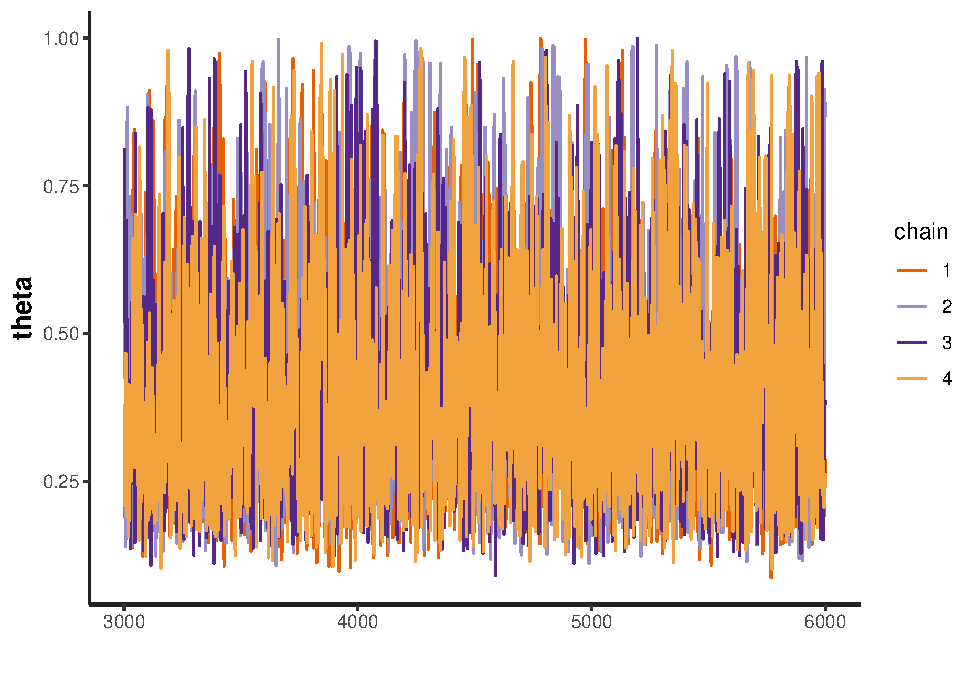
\includegraphics{besvarels_files/figure-latex/unnamed-chunk-16-1.pdf}
The chains seem to be well-mixing. We do not see anything alarming -
i.e.~we do not see anything systematic trends within chains over time
and we do not see differences between chains. We print a summary of the
model

\begin{Shaded}
\begin{Highlighting}[]
\NormalTok{stan\_fit}
\end{Highlighting}
\end{Shaded}

\begin{verbatim}
## Inference for Stan model: anon_model.
## 4 chains, each with iter=6000; warmup=3000; thin=1; 
## post-warmup draws per chain=3000, total post-warmup draws=12000.
## 
##        mean se_mean   sd  2.5%   25%   50%   75% 97.5% n_eff Rhat
## theta  0.42    0.00 0.19  0.16  0.27  0.37  0.53  0.89  2178    1
## lp__  -0.98    0.02 0.88 -3.61 -1.18 -0.63 -0.40 -0.34  2132    1
## 
## Samples were drawn using NUTS(diag_e) at Wed Jan 24 13:00:13 2024.
## For each parameter, n_eff is a crude measure of effective sample size,
## and Rhat is the potential scale reduction factor on split chains (at 
## convergence, Rhat=1).
\end{verbatim}

We see that \(\hat{R}\) for \(\theta\) is 1, indicating that the chains
have converged to their stationary distribution.

\hypertarget{section-11}{%
\subsection{2.}\label{section-11}}

We simulate from the posterior predictive distribution of \(\tilde{Y}\)
by using our simulated values of \(\theta\) from \(\theta\)'s posterior
distribution to simulate from the conditional
\(Y | \theta = \theta' \sim \mathcal{N}(0,\theta')\).

\begin{Shaded}
\begin{Highlighting}[]
\FunctionTok{set.seed}\NormalTok{(}\DecValTok{1}\NormalTok{)}
\NormalTok{theta }\OtherTok{\textless{}{-}} \FunctionTok{extract}\NormalTok{(stan\_fit)}\SpecialCharTok{$}\NormalTok{theta}
\NormalTok{y\_post }\OtherTok{\textless{}{-}} \FunctionTok{rnorm}\NormalTok{(}\FunctionTok{length}\NormalTok{(theta) , }\DecValTok{0}\NormalTok{, theta}\SpecialCharTok{\^{}}\DecValTok{2}\NormalTok{)}
\end{Highlighting}
\end{Shaded}

Say that researchers observe \(y = 1.4\). The probability of observing
something as extreme as 1.4 in the posterior predictive distribution is

\begin{Shaded}
\begin{Highlighting}[]
\FunctionTok{mean}\NormalTok{(y\_post }\SpecialCharTok{\textgreater{}} \FloatTok{1.4}\NormalTok{)}
\end{Highlighting}
\end{Shaded}

\begin{verbatim}
## [1] 0.00275
\end{verbatim}

Which must be considered fairly extreme. This would indicate that the
conditions for the experiment has indeed changed as the researchers are
concerned about.

\end{document}
